\documentclass[twoside]{book}

% Packages required by doxygen
\usepackage{fixltx2e}
\usepackage{calc}
\usepackage{doxygen}
\usepackage[export]{adjustbox} % also loads graphicx
\usepackage{graphicx}
\usepackage[utf8]{inputenc}
\usepackage{makeidx}
\usepackage{multicol}
\usepackage{multirow}
\PassOptionsToPackage{warn}{textcomp}
\usepackage{textcomp}
\usepackage[nointegrals]{wasysym}
\usepackage[table]{xcolor}

% Font selection
\usepackage[T1]{fontenc}
\usepackage[scaled=.90]{helvet}
\usepackage{courier}
\usepackage{amssymb}
\usepackage{sectsty}
\renewcommand{\familydefault}{\sfdefault}
\allsectionsfont{%
  \fontseries{bc}\selectfont%
  \color{darkgray}%
}
\renewcommand{\DoxyLabelFont}{%
  \fontseries{bc}\selectfont%
  \color{darkgray}%
}
\newcommand{\+}{\discretionary{\mbox{\scriptsize$\hookleftarrow$}}{}{}}

% Page & text layout
\usepackage{geometry}
\geometry{%
  a4paper,%
  top=2.5cm,%
  bottom=2.5cm,%
  left=2.5cm,%
  right=2.5cm%
}
\tolerance=750
\hfuzz=15pt
\hbadness=750
\setlength{\emergencystretch}{15pt}
\setlength{\parindent}{0cm}
\setlength{\parskip}{3ex plus 2ex minus 2ex}
\makeatletter
\renewcommand{\paragraph}{%
  \@startsection{paragraph}{4}{0ex}{-1.0ex}{1.0ex}{%
    \normalfont\normalsize\bfseries\SS@parafont%
  }%
}
\renewcommand{\subparagraph}{%
  \@startsection{subparagraph}{5}{0ex}{-1.0ex}{1.0ex}{%
    \normalfont\normalsize\bfseries\SS@subparafont%
  }%
}
\makeatother

% Headers & footers
\usepackage{fancyhdr}
\pagestyle{fancyplain}
\fancyhead[LE]{\fancyplain{}{\bfseries\thepage}}
\fancyhead[CE]{\fancyplain{}{}}
\fancyhead[RE]{\fancyplain{}{\bfseries\leftmark}}
\fancyhead[LO]{\fancyplain{}{\bfseries\rightmark}}
\fancyhead[CO]{\fancyplain{}{}}
\fancyhead[RO]{\fancyplain{}{\bfseries\thepage}}
\fancyfoot[LE]{\fancyplain{}{}}
\fancyfoot[CE]{\fancyplain{}{}}
\fancyfoot[RE]{\fancyplain{}{\bfseries\scriptsize Generated by Doxygen }}
\fancyfoot[LO]{\fancyplain{}{\bfseries\scriptsize Generated by Doxygen }}
\fancyfoot[CO]{\fancyplain{}{}}
\fancyfoot[RO]{\fancyplain{}{}}
\renewcommand{\footrulewidth}{0.4pt}
\renewcommand{\chaptermark}[1]{%
  \markboth{#1}{}%
}
\renewcommand{\sectionmark}[1]{%
  \markright{\thesection\ #1}%
}

% Indices & bibliography
\usepackage{natbib}
\usepackage[titles]{tocloft}
\setcounter{tocdepth}{3}
\setcounter{secnumdepth}{5}
\makeindex

% Custom commands
\newcommand{\clearemptydoublepage}{%
  \newpage{\pagestyle{empty}\cleardoublepage}%
}

\usepackage{caption}
\captionsetup{labelsep=space,justification=centering,font={bf},singlelinecheck=off,skip=4pt,position=top}

%===== C O N T E N T S =====

\begin{document}

% Titlepage & ToC
\pagenumbering{alph}
\begin{titlepage}
\vspace*{7cm}
\begin{center}%
{\Large Packag\+ED }\\
\vspace*{1cm}
{\large Generated by Doxygen 1.8.14}\\
\end{center}
\end{titlepage}
\clearemptydoublepage
\pagenumbering{roman}
\tableofcontents
\clearemptydoublepage
\pagenumbering{arabic}

%--- Begin generated contents ---
\chapter{Packag\+ED}
\label{md__g_1_compu__c_o_p290__packag_e_d__r_e_a_d_m_e}
This repository holds the documentation and code for the assignment in the Course C\+O\+P290 (Design Practices). The aim is to develop a software package for Engineering Drawing.

The package is supposed to have the following functionalities\+:
\begin{DoxyEnumerate}
\item We should be able to interactively input or read from a file either i) an isometric drawing and a 3D object model or ii) projections on to any cross section.
\item Given the 3D model description we should be able to generate projections on to any cross section or cutting plane.
\item Given two or more projections we should be able to interactively recover the 3D description and produce an isometric drawing from any view direction.
\end{DoxyEnumerate}

The package structure for the software package is as follows\+: ~\newline
Packag\+ED $\vert$ ~\newline
 $\vert$-\/$>$ bin ~\newline
 $\vert$-\/$>$ build ~\newline
 $\vert$-\/$>$ doc ~\newline
 $\vert$-\/$>$ include ~\newline
 $\vert$-\/$>$ lib ~\newline
 $\vert$-\/$>$ src ~\newline
 $\vert$-\/$>$ test ~\newline


Following is a description of the above-\/mentioned directories\+:
\begin{DoxyEnumerate}
\item {\bfseries bin} -\/ All the object files, obtained after build shall be kept in this folder.
\item {\bfseries build} -\/ All executables are supposed to be kept in this folder.
\item {\bfseries doc} -\/ All doxygen generated html pages and other documentations relating to the project are supposed to be kept in this folder.
\item {\bfseries include} -\/ All header files to be included in the project are kept in this folder.
\item {\bfseries lib} -\/ This folder contains all external libraries required for the software.
\item {\bfseries src} -\/ This folder is supposed to contain all source files (.cpp) written in C++ are to be kept here.
\item {\bfseries test} -\/ This folder shall be host to all test files written for debugging and testing the software package (yet to be updated). 
\end{DoxyEnumerate}
\chapter{Class Index}
\section{Class List}
Here are the classes, structs, unions and interfaces with brief descriptions\+:\begin{DoxyCompactList}
\item\contentsline{section}{\hyperlink{class_edge}{Edge} }{\pageref{class_edge}}{}
\item\contentsline{section}{\hyperlink{class_face}{Face} }{\pageref{class_face}}{}
\item\contentsline{section}{\hyperlink{class_object3_d}{Object3D} }{\pageref{class_object3_d}}{}
\item\contentsline{section}{\hyperlink{class_ortho_projection}{Ortho\+Projection} }{\pageref{class_ortho_projection}}{}
\item\contentsline{section}{\hyperlink{class_point}{Point} }{\pageref{class_point}}{}
\item\contentsline{section}{\hyperlink{class_projection2_d}{Projection2D} }{\pageref{class_projection2_d}}{}
\item\contentsline{section}{\hyperlink{class_wireframe}{Wireframe} }{\pageref{class_wireframe}}{}
\end{DoxyCompactList}

\chapter{File Index}
\section{File List}
Here is a list of all files with brief descriptions\+:\begin{DoxyCompactList}
\item\contentsline{section}{G\+:/compu/\+C\+O\+P290/\+Packag\+E\+D/include/\textbf{ Classes.\+h} }{\pageref{include_2_classes_8h}}{}
\item\contentsline{section}{G\+:/compu/\+C\+O\+P290/\+Packag\+E\+D/src/\textbf{ check.\+cpp} }{\pageref{check_8cpp}}{}
\item\contentsline{section}{G\+:/compu/\+C\+O\+P290/\+Packag\+E\+D/src/\textbf{ Classes.\+h} }{\pageref{src_2_classes_8h}}{}
\item\contentsline{section}{G\+:/compu/\+C\+O\+P290/\+Packag\+E\+D/src/\textbf{ Main.\+cpp} }{\pageref{_main_8cpp}}{}
\item\contentsline{section}{G\+:/compu/\+C\+O\+P290/\+Packag\+E\+D/src/\textbf{ Object3\+D.\+cpp} }{\pageref{_object3_d_8cpp}}{}
\item\contentsline{section}{G\+:/compu/\+C\+O\+P290/\+Packag\+E\+D/src/\textbf{ Ortho\+Projection.\+cpp} }{\pageref{_ortho_projection_8cpp}}{}
\item\contentsline{section}{G\+:/compu/\+C\+O\+P290/\+Packag\+E\+D/src/\textbf{ Point.\+cpp} }{\pageref{_point_8cpp}}{}
\item\contentsline{section}{G\+:/compu/\+C\+O\+P290/\+Packag\+E\+D/src/\textbf{ Projection2\+D.\+cpp} }{\pageref{_projection2_d_8cpp}}{}
\end{DoxyCompactList}

\chapter{Class Documentation}
\section{check Class Reference}
\label{classcheck}\index{check@{check}}
\subsection*{Public Member Functions}
\begin{DoxyCompactItemize}
\item 
\textbf{ check} \textbf{ function} ()
\end{DoxyCompactItemize}
\subsection*{Public Attributes}
\begin{DoxyCompactItemize}
\item 
int \textbf{ y}
\end{DoxyCompactItemize}


\subsection{Member Function Documentation}
\mbox{\label{classcheck_aea4fe5c31fa6a2b8798e1fc5de71ec95}} 
\index{check@{check}!function@{function}}
\index{function@{function}!check@{check}}
\subsubsection{function()}
{\footnotesize\ttfamily \textbf{ check} check\+::function (\begin{DoxyParamCaption}{ }\end{DoxyParamCaption})}



\subsection{Member Data Documentation}
\mbox{\label{classcheck_acb8c9192a576a58bf4fb8cdbfc326271}} 
\index{check@{check}!y@{y}}
\index{y@{y}!check@{check}}
\subsubsection{y}
{\footnotesize\ttfamily int check\+::y}



The documentation for this class was generated from the following file\+:\begin{DoxyCompactItemize}
\item 
G\+:/compu/\+C\+O\+P290/\+Packag\+E\+D/src/\textbf{ check.\+cpp}\end{DoxyCompactItemize}

\hypertarget{class_edge}{}\section{Edge Class Reference}
\label{class_edge}\index{Edge@{Edge}}


{\ttfamily \#include $<$Classes.\+h$>$}

\subsection*{Public Attributes}
\begin{DoxyCompactItemize}
\item 
\hyperlink{class_point}{Point} \hyperlink{class_edge_a9cb958550d6ca42fd7122235d64898c9}{p1}
\item 
\hyperlink{class_point}{Point} \hyperlink{class_edge_a0867d7b428491ef61eb90b540a73db1d}{p2}
\end{DoxyCompactItemize}


\subsection{Detailed Description}
This class is an abstraction of the edge of a 3D object. It consists of two endpoints (of the type \hyperlink{class_point}{Point}). 

\subsection{Member Data Documentation}
\index{Edge@{Edge}!p1@{p1}}
\index{p1@{p1}!Edge@{Edge}}
\subsubsection[{\texorpdfstring{p1}{p1}}]{\setlength{\rightskip}{0pt plus 5cm}{\bf Point} Edge\+::p1}\hypertarget{class_edge_a9cb958550d6ca42fd7122235d64898c9}{}\label{class_edge_a9cb958550d6ca42fd7122235d64898c9}
\index{Edge@{Edge}!p2@{p2}}
\index{p2@{p2}!Edge@{Edge}}
\subsubsection[{\texorpdfstring{p2}{p2}}]{\setlength{\rightskip}{0pt plus 5cm}{\bf Point} Edge\+::p2}\hypertarget{class_edge_a0867d7b428491ef61eb90b540a73db1d}{}\label{class_edge_a0867d7b428491ef61eb90b540a73db1d}


The documentation for this class was generated from the following file\+:\begin{DoxyCompactItemize}
\item 
Packag\+E\+D/include/\hyperlink{_classes_8h}{Classes.\+h}\end{DoxyCompactItemize}

\hypertarget{class_face}{}\section{Face Class Reference}
\label{class_face}\index{Face@{Face}}


{\ttfamily \#include $<$Classes.\+h$>$}

\subsection*{Public Attributes}
\begin{DoxyCompactItemize}
\item 
\hyperlink{class_point}{Point} \hyperlink{class_face_acb5b50d81748e6dcbab0a533b336f534}{vertices} \mbox{[}$\,$\mbox{]}
\end{DoxyCompactItemize}


\subsection{Detailed Description}
This class is the abstraction to represent the faces of a 3D object. 

\subsection{Member Data Documentation}
\index{Face@{Face}!vertices@{vertices}}
\index{vertices@{vertices}!Face@{Face}}
\subsubsection[{\texorpdfstring{vertices}{vertices}}]{\setlength{\rightskip}{0pt plus 5cm}{\bf Point} Face\+::vertices\mbox{[}$\,$\mbox{]}}\hypertarget{class_face_acb5b50d81748e6dcbab0a533b336f534}{}\label{class_face_acb5b50d81748e6dcbab0a533b336f534}


The documentation for this class was generated from the following file\+:\begin{DoxyCompactItemize}
\item 
Packag\+E\+D/include/\hyperlink{_classes_8h}{Classes.\+h}\end{DoxyCompactItemize}

\hypertarget{class_object3_d}{}\section{Object3D Class Reference}
\label{class_object3_d}\index{Object3D@{Object3D}}


{\ttfamily \#include $<$Classes.\+h$>$}

\subsection*{Public Member Functions}
\begin{DoxyCompactItemize}
\item 
int \hyperlink{class_object3_d_a17e177a936a71e0a5599ce7ca76bae78}{project3D} (double\mbox{[}4\mbox{]})
\item 
\hyperlink{class_object3_d}{Object3D} \hyperlink{class_object3_d_a476b3de610cb30be0b050b4701ba4701}{rotate\+Object} (double, double, double)
\item 
\hyperlink{class_object3_d}{Object3D} \hyperlink{class_object3_d_afb299c53794e9f4fb708efbde24c9a21}{translate} (double, double, double)
\end{DoxyCompactItemize}
\subsection*{Public Attributes}
\begin{DoxyCompactItemize}
\item 
\hyperlink{class_point}{Point} \hyperlink{class_object3_d_a23cc82ea4ef0af8e0e22871bdbdba6c6}{vertices} \mbox{[}$\,$\mbox{]}
\item 
\hyperlink{class_edge}{Edge} \hyperlink{class_object3_d_ad93f210748663a4d0aaa89287dee3dae}{edges} \mbox{[}$\,$\mbox{]}
\item 
\hyperlink{class_face}{Face} \hyperlink{class_object3_d_a4cc7f57059a990a8573a7644a4d3ab2a}{faces} \mbox{[}$\,$\mbox{]}
\end{DoxyCompactItemize}


\subsection{Detailed Description}
This class provides an abstraction for a real world 3D object and incorporates the functions for the same. The class incorporates functions for operating upon the object 

\subsection{Member Function Documentation}
\index{Object3D@{Object3D}!project3D@{project3D}}
\index{project3D@{project3D}!Object3D@{Object3D}}
\subsubsection[{\texorpdfstring{project3\+D(double[4])}{project3D(double[4])}}]{\setlength{\rightskip}{0pt plus 5cm}int Object3\+D\+::project3D (
\begin{DoxyParamCaption}
\item[{double}]{projection\+Plane\mbox{[}4\mbox{]}}
\end{DoxyParamCaption}
)}\hypertarget{class_object3_d_a17e177a936a71e0a5599ce7ca76bae78}{}\label{class_object3_d_a17e177a936a71e0a5599ce7ca76bae78}
General Function to project the current 3D object onto the projection plane passed as parameter \char`\"{}projection\+Plane\char`\"{}\index{Object3D@{Object3D}!rotate\+Object@{rotate\+Object}}
\index{rotate\+Object@{rotate\+Object}!Object3D@{Object3D}}
\subsubsection[{\texorpdfstring{rotate\+Object(double, double, double)}{rotateObject(double, double, double)}}]{\setlength{\rightskip}{0pt plus 5cm}{\bf Object3D} Object3\+D\+::rotate\+Object (
\begin{DoxyParamCaption}
\item[{double}]{aboutx, }
\item[{double}]{abouty, }
\item[{double}]{aboutz}
\end{DoxyParamCaption}
)}\hypertarget{class_object3_d_a476b3de610cb30be0b050b4701ba4701}{}\label{class_object3_d_a476b3de610cb30be0b050b4701ba4701}
Returns a new 3D Object with the rotated coordinates, obtained by rotating the current object by the angles \char`\"{}aboutz\char`\"{} about the Z-\/axis, by \char`\"{}aboutx\char`\"{} about the X-\/axis and by \char`\"{}abouty\char`\"{} about the Y-\/axis\index{Object3D@{Object3D}!translate@{translate}}
\index{translate@{translate}!Object3D@{Object3D}}
\subsubsection[{\texorpdfstring{translate(double, double, double)}{translate(double, double, double)}}]{\setlength{\rightskip}{0pt plus 5cm}{\bf Object3D} Object3\+D\+::translate (
\begin{DoxyParamCaption}
\item[{double}]{x, }
\item[{double}]{y, }
\item[{double}]{z}
\end{DoxyParamCaption}
)}\hypertarget{class_object3_d_afb299c53794e9f4fb708efbde24c9a21}{}\label{class_object3_d_afb299c53794e9f4fb708efbde24c9a21}
This function returns a new \hyperlink{class_object3_d}{Object3D} instance, which is obtained by translating the current object by the distances, specified in the parameters

\subsection{Member Data Documentation}
\index{Object3D@{Object3D}!edges@{edges}}
\index{edges@{edges}!Object3D@{Object3D}}
\subsubsection[{\texorpdfstring{edges}{edges}}]{\setlength{\rightskip}{0pt plus 5cm}{\bf Edge} Object3\+D\+::edges\mbox{[}$\,$\mbox{]}}\hypertarget{class_object3_d_ad93f210748663a4d0aaa89287dee3dae}{}\label{class_object3_d_ad93f210748663a4d0aaa89287dee3dae}
\index{Object3D@{Object3D}!faces@{faces}}
\index{faces@{faces}!Object3D@{Object3D}}
\subsubsection[{\texorpdfstring{faces}{faces}}]{\setlength{\rightskip}{0pt plus 5cm}{\bf Face} Object3\+D\+::faces\mbox{[}$\,$\mbox{]}}\hypertarget{class_object3_d_a4cc7f57059a990a8573a7644a4d3ab2a}{}\label{class_object3_d_a4cc7f57059a990a8573a7644a4d3ab2a}
\index{Object3D@{Object3D}!vertices@{vertices}}
\index{vertices@{vertices}!Object3D@{Object3D}}
\subsubsection[{\texorpdfstring{vertices}{vertices}}]{\setlength{\rightskip}{0pt plus 5cm}{\bf Point} Object3\+D\+::vertices\mbox{[}$\,$\mbox{]}}\hypertarget{class_object3_d_a23cc82ea4ef0af8e0e22871bdbdba6c6}{}\label{class_object3_d_a23cc82ea4ef0af8e0e22871bdbdba6c6}


The documentation for this class was generated from the following files\+:\begin{DoxyCompactItemize}
\item 
Packag\+E\+D/include/\hyperlink{_classes_8h}{Classes.\+h}\item 
Packag\+E\+D/src/\hyperlink{_object3_d_8cpp}{Object3\+D.\+cpp}\end{DoxyCompactItemize}

\hypertarget{class_ortho_projection}{}\section{Ortho\+Projection Class Reference}
\label{class_ortho_projection}\index{Ortho\+Projection@{Ortho\+Projection}}


{\ttfamily \#include $<$Classes.\+h$>$}

\subsection*{Public Member Functions}
\begin{DoxyCompactItemize}
\item 
\hyperlink{class_point}{Point} $\ast$ \hyperlink{class_ortho_projection_aa0634b80a904634451f03a11db28c33d}{possible\+Neighbours} (\hyperlink{class_point}{Point})
\end{DoxyCompactItemize}
\subsection*{Public Attributes}
\begin{DoxyCompactItemize}
\item 
\hyperlink{class_point}{Point} \hyperlink{class_ortho_projection_a66b7e72014671cf35f4c6728b7baeec6}{vertices} \mbox{[}$\,$\mbox{]}
\item 
\hyperlink{class_edge}{Edge} \hyperlink{class_ortho_projection_a8903896a5a8facc50585ea50584617a1}{visible\+Edges} \mbox{[}$\,$\mbox{]}
\item 
\hyperlink{class_edge}{Edge} \hyperlink{class_ortho_projection_af5ebfefeb5cbc7ba0373697161ce27da}{hidden\+Edges} \mbox{[}$\,$\mbox{]}
\end{DoxyCompactItemize}


\subsection{Detailed Description}
This class provides an abstraction for the 2D projection of a 3D object on a plane. 

\subsection{Member Function Documentation}
\index{Ortho\+Projection@{Ortho\+Projection}!possible\+Neighbours@{possible\+Neighbours}}
\index{possible\+Neighbours@{possible\+Neighbours}!Ortho\+Projection@{Ortho\+Projection}}
\subsubsection[{\texorpdfstring{possible\+Neighbours(\+Point)}{possibleNeighbours(Point)}}]{\setlength{\rightskip}{0pt plus 5cm}{\bf Point} $\ast$ Ortho\+Projection\+::possible\+Neighbours (
\begin{DoxyParamCaption}
\item[{{\bf Point}}]{point}
\end{DoxyParamCaption}
)}\hypertarget{class_ortho_projection_aa0634b80a904634451f03a11db28c33d}{}\label{class_ortho_projection_aa0634b80a904634451f03a11db28c33d}
Function that returns a list of possible neighbors of the point passed in parameter, from the current orthographic projection

\subsection{Member Data Documentation}
\index{Ortho\+Projection@{Ortho\+Projection}!hidden\+Edges@{hidden\+Edges}}
\index{hidden\+Edges@{hidden\+Edges}!Ortho\+Projection@{Ortho\+Projection}}
\subsubsection[{\texorpdfstring{hidden\+Edges}{hiddenEdges}}]{\setlength{\rightskip}{0pt plus 5cm}{\bf Edge} Ortho\+Projection\+::hidden\+Edges\mbox{[}$\,$\mbox{]}}\hypertarget{class_ortho_projection_af5ebfefeb5cbc7ba0373697161ce27da}{}\label{class_ortho_projection_af5ebfefeb5cbc7ba0373697161ce27da}
\index{Ortho\+Projection@{Ortho\+Projection}!vertices@{vertices}}
\index{vertices@{vertices}!Ortho\+Projection@{Ortho\+Projection}}
\subsubsection[{\texorpdfstring{vertices}{vertices}}]{\setlength{\rightskip}{0pt plus 5cm}{\bf Point} Ortho\+Projection\+::vertices\mbox{[}$\,$\mbox{]}}\hypertarget{class_ortho_projection_a66b7e72014671cf35f4c6728b7baeec6}{}\label{class_ortho_projection_a66b7e72014671cf35f4c6728b7baeec6}
\index{Ortho\+Projection@{Ortho\+Projection}!visible\+Edges@{visible\+Edges}}
\index{visible\+Edges@{visible\+Edges}!Ortho\+Projection@{Ortho\+Projection}}
\subsubsection[{\texorpdfstring{visible\+Edges}{visibleEdges}}]{\setlength{\rightskip}{0pt plus 5cm}{\bf Edge} Ortho\+Projection\+::visible\+Edges\mbox{[}$\,$\mbox{]}}\hypertarget{class_ortho_projection_a8903896a5a8facc50585ea50584617a1}{}\label{class_ortho_projection_a8903896a5a8facc50585ea50584617a1}


The documentation for this class was generated from the following files\+:\begin{DoxyCompactItemize}
\item 
Packag\+E\+D/include/\hyperlink{_classes_8h}{Classes.\+h}\item 
Packag\+E\+D/src/\hyperlink{_ortho_projection_8cpp}{Ortho\+Projection.\+cpp}\end{DoxyCompactItemize}

\hypertarget{class_point}{}\section{Point Class Reference}
\label{class_point}\index{Point@{Point}}


{\ttfamily \#include $<$Classes.\+h$>$}

\subsection*{Public Member Functions}
\begin{DoxyCompactItemize}
\item 
\hyperlink{class_point}{Point} \hyperlink{class_point_a209c076529495ad94cf65b8a71d29913}{project\+Point} (double\mbox{[}$\,$\mbox{]})
\item 
double \hyperlink{class_point_a700201e1da138be7e3225b9d2bff50e9}{relative\+Position} (double\mbox{[}$\,$\mbox{]})
\end{DoxyCompactItemize}
\subsection*{Public Attributes}
\begin{DoxyCompactItemize}
\item 
double \hyperlink{class_point_ab99c56589bc8ad5fa5071387110a5bc7}{x}
\item 
double \hyperlink{class_point_afa38be143ae800e6ad69ce8ed4df62d8}{y}
\item 
double \hyperlink{class_point_a05ba3b1dfcb19430582ae953cbbfbded}{z}
\end{DoxyCompactItemize}


\subsection{Detailed Description}
This class is an abstraction of a real-\/world 3D point. 

\subsection{Member Function Documentation}
\index{Point@{Point}!project\+Point@{project\+Point}}
\index{project\+Point@{project\+Point}!Point@{Point}}
\subsubsection[{\texorpdfstring{project\+Point(double[])}{projectPoint(double[])}}]{\setlength{\rightskip}{0pt plus 5cm}{\bf Point} Point\+::project\+Point (
\begin{DoxyParamCaption}
\item[{double}]{projection\+Plane\mbox{[}$\,$\mbox{]}}
\end{DoxyParamCaption}
)}\hypertarget{class_point_a209c076529495ad94cf65b8a71d29913}{}\label{class_point_a209c076529495ad94cf65b8a71d29913}
Function to give the projection of the current calling object on the projection plane passed in parameters as \char`\"{}projection\+Plane\char`\"{}\index{Point@{Point}!relative\+Position@{relative\+Position}}
\index{relative\+Position@{relative\+Position}!Point@{Point}}
\subsubsection[{\texorpdfstring{relative\+Position(double[])}{relativePosition(double[])}}]{\setlength{\rightskip}{0pt plus 5cm}double Point\+::relative\+Position (
\begin{DoxyParamCaption}
\item[{double}]{plane\mbox{[}$\,$\mbox{]}}
\end{DoxyParamCaption}
)}\hypertarget{class_point_a700201e1da138be7e3225b9d2bff50e9}{}\label{class_point_a700201e1da138be7e3225b9d2bff50e9}
Function to calculate the relative position of the current calling object w.\+r.\+t the passed parameter \char`\"{}plane\char`\"{}

\subsection{Member Data Documentation}
\index{Point@{Point}!x@{x}}
\index{x@{x}!Point@{Point}}
\subsubsection[{\texorpdfstring{x}{x}}]{\setlength{\rightskip}{0pt plus 5cm}double Point\+::x}\hypertarget{class_point_ab99c56589bc8ad5fa5071387110a5bc7}{}\label{class_point_ab99c56589bc8ad5fa5071387110a5bc7}
\index{Point@{Point}!y@{y}}
\index{y@{y}!Point@{Point}}
\subsubsection[{\texorpdfstring{y}{y}}]{\setlength{\rightskip}{0pt plus 5cm}double Point\+::y}\hypertarget{class_point_afa38be143ae800e6ad69ce8ed4df62d8}{}\label{class_point_afa38be143ae800e6ad69ce8ed4df62d8}
\index{Point@{Point}!z@{z}}
\index{z@{z}!Point@{Point}}
\subsubsection[{\texorpdfstring{z}{z}}]{\setlength{\rightskip}{0pt plus 5cm}double Point\+::z}\hypertarget{class_point_a05ba3b1dfcb19430582ae953cbbfbded}{}\label{class_point_a05ba3b1dfcb19430582ae953cbbfbded}


The documentation for this class was generated from the following files\+:\begin{DoxyCompactItemize}
\item 
Packag\+E\+D/include/\hyperlink{_classes_8h}{Classes.\+h}\item 
Packag\+E\+D/src/\hyperlink{_point_8cpp}{Point.\+cpp}\end{DoxyCompactItemize}

\hypertarget{class_projection2_d}{}\section{Projection2D Class Reference}
\label{class_projection2_d}\index{Projection2D@{Projection2D}}


{\ttfamily \#include $<$Classes.\+h$>$}



Collaboration diagram for Projection2D\+:\nopagebreak
\begin{figure}[H]
\begin{center}
\leavevmode
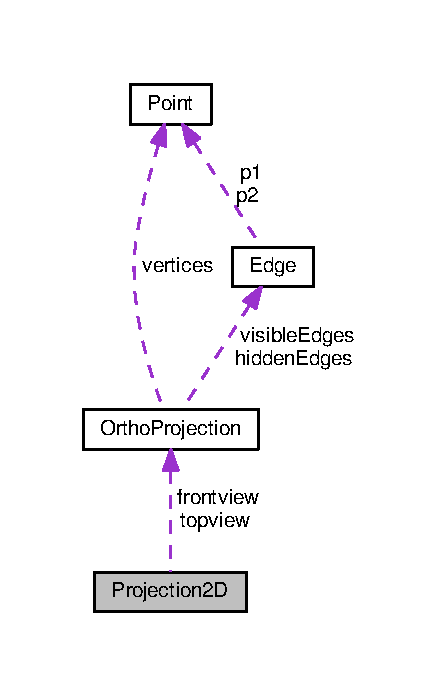
\includegraphics[width=165pt]{class_projection2_d__coll__graph}
\end{center}
\end{figure}
\subsection*{Public Member Functions}
\begin{DoxyCompactItemize}
\item 
\hyperlink{class_wireframe}{Wireframe} \hyperlink{class_projection2_d_aa061602930f19acad32720f7067c58fa}{create3D} ()
\item 
void \hyperlink{class_projection2_d_a64751fc8527786d489d3e1f9dd613778}{chkif3edgesanddefthem} ()
\item 
void \hyperlink{class_projection2_d_a6be4ef41d013628ba91a3f1dbcc1f9bf}{determine\+Intersected\+Edges} ()
\item 
void \hyperlink{class_projection2_d_af65b18c0f1aed2c6bda79173ef6a0f5e}{execute\+Corollary1onebyone} (\hyperlink{class_ortho_projection}{Ortho\+Projection} $\ast$, \hyperlink{class_ortho_projection}{Ortho\+Projection} $\ast$, \hyperlink{class_ortho_projection}{Ortho\+Projection} $\ast$)
\item 
void \hyperlink{class_projection2_d_a7433a1a25a81f16a79c308d5dd7d98b5}{execute\+Corollary1} ()
\item 
\hyperlink{class_point}{Point} \hyperlink{class_projection2_d_a0185949b0711aa0a43bd2f66da9aaee7}{determine\+Point} (\hyperlink{class_point}{Point}, \hyperlink{class_point}{Point})
\item 
vector$<$ \hyperlink{class_point}{Point} $>$ \hyperlink{class_projection2_d_af2972a56d0f0fa6a9d01576d7021180d}{determine\+All\+Points} ()
\item 
pair$<$ vector$<$ \hyperlink{class_edge}{Edge} $>$, vector$<$ vector$<$ int $>$ $>$ $>$ \hyperlink{class_projection2_d_ad5f6fe26ce1a18cb5de2fe87e6b0869e}{determine\+Possible\+Edges} (\hyperlink{class_point}{Point}, vector$<$ \hyperlink{class_point}{Point} $>$ $\ast$, vector$<$ \hyperlink{class_point}{Point} $>$ $\ast$)
\item 
int \hyperlink{class_projection2_d_ad277ae374c9340f41f821e3b23aa6c04}{numofpossibleedge} ()
\item 
bool \hyperlink{class_projection2_d_af9a959f2c44a1801687dda170ba0d5d2}{chkcollinearpossanddef} ()
\item 
bool \hyperlink{class_projection2_d_a26179e263ee8be9bfbc260bedaea14c7}{chkcollinearpossandposs} ()
\item 
bool \hyperlink{class_projection2_d_a7b26c1f31633d19a33bdf54e8c47d3d8}{chkposshasdefinother} ()
\item 
void \hyperlink{class_projection2_d_a209abc191321c5bdd970c57c68dd0ac8}{printmatrix} (vector$<$ vector$<$ int $>$ $>$)
\item 
vector$<$ int $>$ \hyperlink{class_projection2_d_ac86b5c70c7ad7d1e3e3df3f41161bec7}{findneighbours} (int)
\item 
vector$<$ vector$<$ int $>$ $>$ \hyperlink{class_projection2_d_a12296093badead168e68c689df080332}{giveallpaths} (int, int)
\item 
void \hyperlink{class_projection2_d_a71696fe8650908a7c0b98e4059d1ecf9}{give\+All\+Paths\+Util} (int, int, bool\mbox{[}$\,$\mbox{]}, int\mbox{[}$\,$\mbox{]}, int \&, vector$<$ vector$<$ int $>$ $>$)
\item 
vector$<$ vector$<$ int $>$ $>$ \hyperlink{class_projection2_d_af623f07691c744da9b1c2df473df858a}{giveplanarpaths} (vector$<$ vector$<$ int $>$ $>$)
\item 
bool \hyperlink{class_projection2_d_a4b86c26f97d2a91f7fde20fa7ab51092}{isplanar} (vector$<$ int $>$)
\end{DoxyCompactItemize}
\subsection*{Public Attributes}
\begin{DoxyCompactItemize}
\item 
\hyperlink{class_ortho_projection}{Ortho\+Projection} \hyperlink{class_projection2_d_a1eb4d010190b1bd62bf0f9c4e4afc88a}{frontview}
\item 
\hyperlink{class_ortho_projection}{Ortho\+Projection} \hyperlink{class_projection2_d_a90079954379a766f60ba01ad393327ab}{topview}
\item 
\hyperlink{class_ortho_projection}{Ortho\+Projection} \hyperlink{class_projection2_d_a82c9e3f197b07ffe9a10f59de60edbee}{sideview}
\item 
vector$<$ \hyperlink{class_point}{Point} $>$ \hyperlink{class_projection2_d_aacafd767e5289005e7ec5d48c791d02f}{allpoints}
\item 
vector$<$ vector$<$ int $>$ $>$ \hyperlink{class_projection2_d_a0a4be368b0a7233a1aa93efe17c7314e}{adjacency\+Matrix}
\item 
map$<$ int, \hyperlink{class_point}{Point} $\ast$ $>$ \hyperlink{class_projection2_d_a08675aad4022218dc78dd54187be18a9}{indextopointmap}
\item 
map$<$ string, \hyperlink{class_point}{Point} $\ast$ $>$ \hyperlink{class_projection2_d_a0afd92ccd321bc86e6e019b4bec99fc8}{labeltopointmap}
\end{DoxyCompactItemize}


\subsection{Detailed Description}
This class holds the 2D orthographic projections of a 3D object. The orthographic views given by the user must be on the standard planes of reference. We describe our model, assuming that\+: 1. Top view is taken on x-\/y plane
\begin{DoxyEnumerate}
\item Front view must be taken on x-\/z plane 
\end{DoxyEnumerate}

\subsection{Member Function Documentation}
\index{Projection2D@{Projection2D}!chkcollinearpossanddef@{chkcollinearpossanddef}}
\index{chkcollinearpossanddef@{chkcollinearpossanddef}!Projection2D@{Projection2D}}
\subsubsection[{\texorpdfstring{chkcollinearpossanddef()}{chkcollinearpossanddef()}}]{\setlength{\rightskip}{0pt plus 5cm}bool Projection2\+D\+::chkcollinearpossanddef (
\begin{DoxyParamCaption}
{}
\end{DoxyParamCaption}
)}\hypertarget{class_projection2_d_af9a959f2c44a1801687dda170ba0d5d2}{}\label{class_projection2_d_af9a959f2c44a1801687dda170ba0d5d2}
check if a point has two collinear points as its edge, one being definite and other being possible, if so, remove the possible edge

Here is the call graph for this function\+:\nopagebreak
\begin{figure}[H]
\begin{center}
\leavevmode
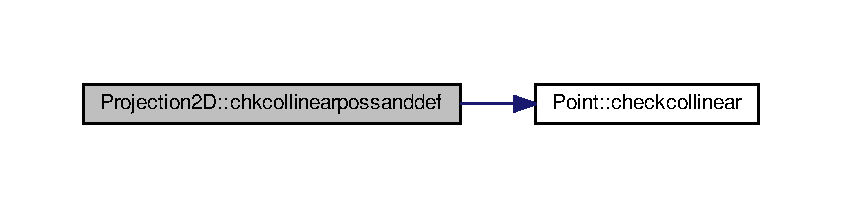
\includegraphics[width=350pt]{class_projection2_d_af9a959f2c44a1801687dda170ba0d5d2_cgraph}
\end{center}
\end{figure}


\index{Projection2D@{Projection2D}!chkcollinearpossandposs@{chkcollinearpossandposs}}
\index{chkcollinearpossandposs@{chkcollinearpossandposs}!Projection2D@{Projection2D}}
\subsubsection[{\texorpdfstring{chkcollinearpossandposs()}{chkcollinearpossandposs()}}]{\setlength{\rightskip}{0pt plus 5cm}bool Projection2\+D\+::chkcollinearpossandposs (
\begin{DoxyParamCaption}
{}
\end{DoxyParamCaption}
)}\hypertarget{class_projection2_d_a26179e263ee8be9bfbc260bedaea14c7}{}\label{class_projection2_d_a26179e263ee8be9bfbc260bedaea14c7}
if two points are collinear and possible edges only one of them could be definite, definite being the closest point, Given that the point whose neighbours are being calculated lies on one end

Here is the call graph for this function\+:\nopagebreak
\begin{figure}[H]
\begin{center}
\leavevmode
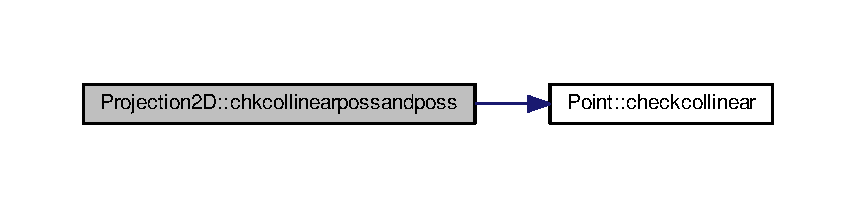
\includegraphics[width=350pt]{class_projection2_d_a26179e263ee8be9bfbc260bedaea14c7_cgraph}
\end{center}
\end{figure}


\index{Projection2D@{Projection2D}!chkif3edgesanddefthem@{chkif3edgesanddefthem}}
\index{chkif3edgesanddefthem@{chkif3edgesanddefthem}!Projection2D@{Projection2D}}
\subsubsection[{\texorpdfstring{chkif3edgesanddefthem()}{chkif3edgesanddefthem()}}]{\setlength{\rightskip}{0pt plus 5cm}void Projection2\+D\+::chkif3edgesanddefthem (
\begin{DoxyParamCaption}
{}
\end{DoxyParamCaption}
)}\hypertarget{class_projection2_d_a64751fc8527786d489d3e1f9dd613778}{}\label{class_projection2_d_a64751fc8527786d489d3e1f9dd613778}
Function to check if there are only three possible edges and then make them the final edge\index{Projection2D@{Projection2D}!chkposshasdefinother@{chkposshasdefinother}}
\index{chkposshasdefinother@{chkposshasdefinother}!Projection2D@{Projection2D}}
\subsubsection[{\texorpdfstring{chkposshasdefinother()}{chkposshasdefinother()}}]{\setlength{\rightskip}{0pt plus 5cm}bool Projection2\+D\+::chkposshasdefinother (
\begin{DoxyParamCaption}
{}
\end{DoxyParamCaption}
)}\hypertarget{class_projection2_d_a7b26c1f31633d19a33bdf54e8c47d3d8}{}\label{class_projection2_d_a7b26c1f31633d19a33bdf54e8c47d3d8}
Function to check if a possible edge point has definite neighbours with other edges, if so remove them\index{Projection2D@{Projection2D}!create3D@{create3D}}
\index{create3D@{create3D}!Projection2D@{Projection2D}}
\subsubsection[{\texorpdfstring{create3\+D()}{create3D()}}]{\setlength{\rightskip}{0pt plus 5cm}{\bf Wireframe} Projection2\+D\+::create3D (
\begin{DoxyParamCaption}
{}
\end{DoxyParamCaption}
)}\hypertarget{class_projection2_d_aa061602930f19acad32720f7067c58fa}{}\label{class_projection2_d_aa061602930f19acad32720f7067c58fa}
Function that creates the wireframe model from the 2d orthographic views\index{Projection2D@{Projection2D}!determine\+All\+Points@{determine\+All\+Points}}
\index{determine\+All\+Points@{determine\+All\+Points}!Projection2D@{Projection2D}}
\subsubsection[{\texorpdfstring{determine\+All\+Points()}{determineAllPoints()}}]{\setlength{\rightskip}{0pt plus 5cm}vector$<$ {\bf Point} $>$ Projection2\+D\+::determine\+All\+Points (
\begin{DoxyParamCaption}
{}
\end{DoxyParamCaption}
)}\hypertarget{class_projection2_d_af2972a56d0f0fa6a9d01576d7021180d}{}\label{class_projection2_d_af2972a56d0f0fa6a9d01576d7021180d}
Function to determine points by intersection of the corresponding points from topview and frontview\index{Projection2D@{Projection2D}!determine\+Intersected\+Edges@{determine\+Intersected\+Edges}}
\index{determine\+Intersected\+Edges@{determine\+Intersected\+Edges}!Projection2D@{Projection2D}}
\subsubsection[{\texorpdfstring{determine\+Intersected\+Edges()}{determineIntersectedEdges()}}]{\setlength{\rightskip}{0pt plus 5cm}void Projection2\+D\+::determine\+Intersected\+Edges (
\begin{DoxyParamCaption}
{}
\end{DoxyParamCaption}
)}\hypertarget{class_projection2_d_a6be4ef41d013628ba91a3f1dbcc1f9bf}{}\label{class_projection2_d_a6be4ef41d013628ba91a3f1dbcc1f9bf}
Funtion to determine all the possible edges for all the points\index{Projection2D@{Projection2D}!determine\+Point@{determine\+Point}}
\index{determine\+Point@{determine\+Point}!Projection2D@{Projection2D}}
\subsubsection[{\texorpdfstring{determine\+Point(\+Point, Point)}{determinePoint(Point, Point)}}]{\setlength{\rightskip}{0pt plus 5cm}{\bf Point} Projection2\+D\+::determine\+Point (
\begin{DoxyParamCaption}
\item[{{\bf Point}}]{pfront, }
\item[{{\bf Point}}]{ptop}
\end{DoxyParamCaption}
)}\hypertarget{class_projection2_d_a0185949b0711aa0a43bd2f66da9aaee7}{}\label{class_projection2_d_a0185949b0711aa0a43bd2f66da9aaee7}
This function extends the points from the top view and front view to give the 3D projection of the \hyperlink{class_point}{Point}

Here is the call graph for this function\+:\nopagebreak
\begin{figure}[H]
\begin{center}
\leavevmode
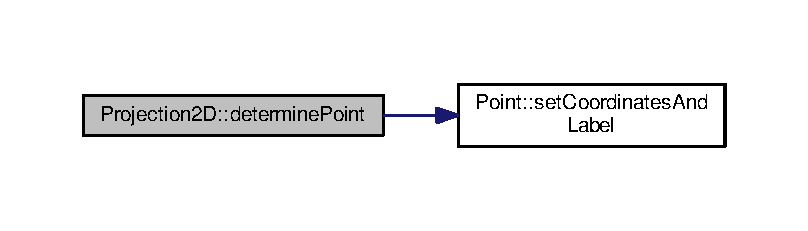
\includegraphics[width=350pt]{class_projection2_d_a0185949b0711aa0a43bd2f66da9aaee7_cgraph}
\end{center}
\end{figure}


\index{Projection2D@{Projection2D}!determine\+Possible\+Edges@{determine\+Possible\+Edges}}
\index{determine\+Possible\+Edges@{determine\+Possible\+Edges}!Projection2D@{Projection2D}}
\subsubsection[{\texorpdfstring{determine\+Possible\+Edges(\+Point, vector$<$ Point $>$ $\ast$, vector$<$ Point $>$ $\ast$)}{determinePossibleEdges(Point, vector< Point > *, vector< Point > *)}}]{\setlength{\rightskip}{0pt plus 5cm}pair$<$ vector$<$ {\bf Edge} $>$, vector$<$ vector$<$ int $>$ $>$ $>$ Projection2\+D\+::determine\+Possible\+Edges (
\begin{DoxyParamCaption}
\item[{{\bf Point}}]{vertex, }
\item[{vector$<$ {\bf Point} $>$ $\ast$}]{topneighbourptr, }
\item[{vector$<$ {\bf Point} $>$ $\ast$}]{frontneighbourptr}
\end{DoxyParamCaption}
)}\hypertarget{class_projection2_d_ad5f6fe26ce1a18cb5de2fe87e6b0869e}{}\label{class_projection2_d_ad5f6fe26ce1a18cb5de2fe87e6b0869e}
This function determines the edges containing the \hyperlink{class_point}{Point} vertex as one of the endpoints By interpreting its neighbours from the top view and front view\index{Projection2D@{Projection2D}!execute\+Corollary1@{execute\+Corollary1}}
\index{execute\+Corollary1@{execute\+Corollary1}!Projection2D@{Projection2D}}
\subsubsection[{\texorpdfstring{execute\+Corollary1()}{executeCorollary1()}}]{\setlength{\rightskip}{0pt plus 5cm}void Projection2\+D\+::execute\+Corollary1 (
\begin{DoxyParamCaption}
{}
\end{DoxyParamCaption}
)}\hypertarget{class_projection2_d_a7433a1a25a81f16a79c308d5dd7d98b5}{}\label{class_projection2_d_a7433a1a25a81f16a79c308d5dd7d98b5}
Function to execute corollary one for all views\index{Projection2D@{Projection2D}!execute\+Corollary1onebyone@{execute\+Corollary1onebyone}}
\index{execute\+Corollary1onebyone@{execute\+Corollary1onebyone}!Projection2D@{Projection2D}}
\subsubsection[{\texorpdfstring{execute\+Corollary1onebyone(\+Ortho\+Projection $\ast$, Ortho\+Projection $\ast$, Ortho\+Projection $\ast$)}{executeCorollary1onebyone(OrthoProjection *, OrthoProjection *, OrthoProjection *)}}]{\setlength{\rightskip}{0pt plus 5cm}void Projection2\+D\+::execute\+Corollary1onebyone (
\begin{DoxyParamCaption}
\item[{{\bf Ortho\+Projection} $\ast$}]{view1, }
\item[{{\bf Ortho\+Projection} $\ast$}]{view2, }
\item[{{\bf Ortho\+Projection} $\ast$}]{view3}
\end{DoxyParamCaption}
)}\hypertarget{class_projection2_d_af65b18c0f1aed2c6bda79173ef6a0f5e}{}\label{class_projection2_d_af65b18c0f1aed2c6bda79173ef6a0f5e}
Function to execute corollary one of superimposed points in one view and possible edge in other view for each view

Here is the call graph for this function\+:\nopagebreak
\begin{figure}[H]
\begin{center}
\leavevmode
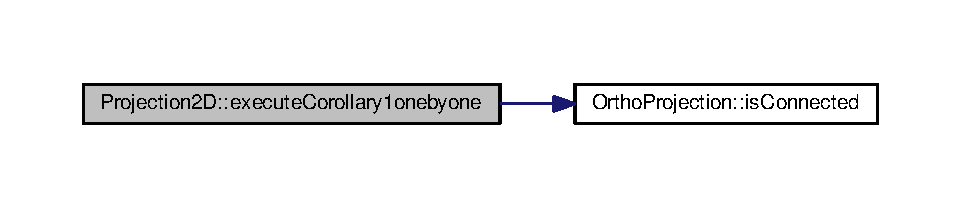
\includegraphics[width=350pt]{class_projection2_d_af65b18c0f1aed2c6bda79173ef6a0f5e_cgraph}
\end{center}
\end{figure}


\index{Projection2D@{Projection2D}!findneighbours@{findneighbours}}
\index{findneighbours@{findneighbours}!Projection2D@{Projection2D}}
\subsubsection[{\texorpdfstring{findneighbours(int)}{findneighbours(int)}}]{\setlength{\rightskip}{0pt plus 5cm}vector$<$ int $>$ Projection2\+D\+::findneighbours (
\begin{DoxyParamCaption}
\item[{int}]{thispoint}
\end{DoxyParamCaption}
)}\hypertarget{class_projection2_d_ac86b5c70c7ad7d1e3e3df3f41161bec7}{}\label{class_projection2_d_ac86b5c70c7ad7d1e3e3df3f41161bec7}
\index{Projection2D@{Projection2D}!giveallpaths@{giveallpaths}}
\index{giveallpaths@{giveallpaths}!Projection2D@{Projection2D}}
\subsubsection[{\texorpdfstring{giveallpaths(int, int)}{giveallpaths(int, int)}}]{\setlength{\rightskip}{0pt plus 5cm}vector$<$vector$<$int$>$ $>$ Projection2\+D\+::giveallpaths (
\begin{DoxyParamCaption}
\item[{int}]{, }
\item[{int}]{}
\end{DoxyParamCaption}
)}\hypertarget{class_projection2_d_a12296093badead168e68c689df080332}{}\label{class_projection2_d_a12296093badead168e68c689df080332}
\index{Projection2D@{Projection2D}!give\+All\+Paths\+Util@{give\+All\+Paths\+Util}}
\index{give\+All\+Paths\+Util@{give\+All\+Paths\+Util}!Projection2D@{Projection2D}}
\subsubsection[{\texorpdfstring{give\+All\+Paths\+Util(int, int, bool[], int[], int \&, vector$<$ vector$<$ int $>$ $>$)}{giveAllPathsUtil(int, int, bool[], int[], int &, vector< vector< int > >)}}]{\setlength{\rightskip}{0pt plus 5cm}void Projection2\+D\+::give\+All\+Paths\+Util (
\begin{DoxyParamCaption}
\item[{int}]{, }
\item[{int}]{, }
\item[{bool}]{\mbox{[}$\,$\mbox{]}, }
\item[{int}]{\mbox{[}$\,$\mbox{]}, }
\item[{int \&}]{, }
\item[{vector$<$ vector$<$ int $>$ $>$}]{}
\end{DoxyParamCaption}
)}\hypertarget{class_projection2_d_a71696fe8650908a7c0b98e4059d1ecf9}{}\label{class_projection2_d_a71696fe8650908a7c0b98e4059d1ecf9}
\index{Projection2D@{Projection2D}!giveplanarpaths@{giveplanarpaths}}
\index{giveplanarpaths@{giveplanarpaths}!Projection2D@{Projection2D}}
\subsubsection[{\texorpdfstring{giveplanarpaths(vector$<$ vector$<$ int $>$ $>$)}{giveplanarpaths(vector< vector< int > >)}}]{\setlength{\rightskip}{0pt plus 5cm}vector$<$vector$<$int$>$ $>$ Projection2\+D\+::giveplanarpaths (
\begin{DoxyParamCaption}
\item[{vector$<$ vector$<$ int $>$ $>$}]{}
\end{DoxyParamCaption}
)}\hypertarget{class_projection2_d_af623f07691c744da9b1c2df473df858a}{}\label{class_projection2_d_af623f07691c744da9b1c2df473df858a}
\index{Projection2D@{Projection2D}!isplanar@{isplanar}}
\index{isplanar@{isplanar}!Projection2D@{Projection2D}}
\subsubsection[{\texorpdfstring{isplanar(vector$<$ int $>$)}{isplanar(vector< int >)}}]{\setlength{\rightskip}{0pt plus 5cm}bool Projection2\+D\+::isplanar (
\begin{DoxyParamCaption}
\item[{vector$<$ int $>$}]{}
\end{DoxyParamCaption}
)}\hypertarget{class_projection2_d_a4b86c26f97d2a91f7fde20fa7ab51092}{}\label{class_projection2_d_a4b86c26f97d2a91f7fde20fa7ab51092}
\index{Projection2D@{Projection2D}!numofpossibleedge@{numofpossibleedge}}
\index{numofpossibleedge@{numofpossibleedge}!Projection2D@{Projection2D}}
\subsubsection[{\texorpdfstring{numofpossibleedge()}{numofpossibleedge()}}]{\setlength{\rightskip}{0pt plus 5cm}int Projection2\+D\+::numofpossibleedge (
\begin{DoxyParamCaption}
{}
\end{DoxyParamCaption}
)}\hypertarget{class_projection2_d_ad277ae374c9340f41f821e3b23aa6c04}{}\label{class_projection2_d_ad277ae374c9340f41f821e3b23aa6c04}
Function to determine possible edges\index{Projection2D@{Projection2D}!printmatrix@{printmatrix}}
\index{printmatrix@{printmatrix}!Projection2D@{Projection2D}}
\subsubsection[{\texorpdfstring{printmatrix(vector$<$ vector$<$ int $>$ $>$)}{printmatrix(vector< vector< int > >)}}]{\setlength{\rightskip}{0pt plus 5cm}void Projection2\+D\+::printmatrix (
\begin{DoxyParamCaption}
\item[{vector$<$ vector$<$ int $>$ $>$}]{thisone}
\end{DoxyParamCaption}
)}\hypertarget{class_projection2_d_a209abc191321c5bdd970c57c68dd0ac8}{}\label{class_projection2_d_a209abc191321c5bdd970c57c68dd0ac8}
Function to print the matrix

\subsection{Member Data Documentation}
\index{Projection2D@{Projection2D}!adjacency\+Matrix@{adjacency\+Matrix}}
\index{adjacency\+Matrix@{adjacency\+Matrix}!Projection2D@{Projection2D}}
\subsubsection[{\texorpdfstring{adjacency\+Matrix}{adjacencyMatrix}}]{\setlength{\rightskip}{0pt plus 5cm}vector$<$vector$<$int$>$ $>$ Projection2\+D\+::adjacency\+Matrix}\hypertarget{class_projection2_d_a0a4be368b0a7233a1aa93efe17c7314e}{}\label{class_projection2_d_a0a4be368b0a7233a1aa93efe17c7314e}
\index{Projection2D@{Projection2D}!allpoints@{allpoints}}
\index{allpoints@{allpoints}!Projection2D@{Projection2D}}
\subsubsection[{\texorpdfstring{allpoints}{allpoints}}]{\setlength{\rightskip}{0pt plus 5cm}vector$<${\bf Point}$>$ Projection2\+D\+::allpoints}\hypertarget{class_projection2_d_aacafd767e5289005e7ec5d48c791d02f}{}\label{class_projection2_d_aacafd767e5289005e7ec5d48c791d02f}
\index{Projection2D@{Projection2D}!frontview@{frontview}}
\index{frontview@{frontview}!Projection2D@{Projection2D}}
\subsubsection[{\texorpdfstring{frontview}{frontview}}]{\setlength{\rightskip}{0pt plus 5cm}{\bf Ortho\+Projection} Projection2\+D\+::frontview}\hypertarget{class_projection2_d_a1eb4d010190b1bd62bf0f9c4e4afc88a}{}\label{class_projection2_d_a1eb4d010190b1bd62bf0f9c4e4afc88a}
\index{Projection2D@{Projection2D}!indextopointmap@{indextopointmap}}
\index{indextopointmap@{indextopointmap}!Projection2D@{Projection2D}}
\subsubsection[{\texorpdfstring{indextopointmap}{indextopointmap}}]{\setlength{\rightskip}{0pt plus 5cm}map$<$int, {\bf Point} $\ast$$>$ Projection2\+D\+::indextopointmap}\hypertarget{class_projection2_d_a08675aad4022218dc78dd54187be18a9}{}\label{class_projection2_d_a08675aad4022218dc78dd54187be18a9}
\index{Projection2D@{Projection2D}!labeltopointmap@{labeltopointmap}}
\index{labeltopointmap@{labeltopointmap}!Projection2D@{Projection2D}}
\subsubsection[{\texorpdfstring{labeltopointmap}{labeltopointmap}}]{\setlength{\rightskip}{0pt plus 5cm}map$<$string, {\bf Point} $\ast$$>$ Projection2\+D\+::labeltopointmap}\hypertarget{class_projection2_d_a0afd92ccd321bc86e6e019b4bec99fc8}{}\label{class_projection2_d_a0afd92ccd321bc86e6e019b4bec99fc8}
\index{Projection2D@{Projection2D}!sideview@{sideview}}
\index{sideview@{sideview}!Projection2D@{Projection2D}}
\subsubsection[{\texorpdfstring{sideview}{sideview}}]{\setlength{\rightskip}{0pt plus 5cm}{\bf Ortho\+Projection} Projection2\+D\+::sideview}\hypertarget{class_projection2_d_a82c9e3f197b07ffe9a10f59de60edbee}{}\label{class_projection2_d_a82c9e3f197b07ffe9a10f59de60edbee}
\index{Projection2D@{Projection2D}!topview@{topview}}
\index{topview@{topview}!Projection2D@{Projection2D}}
\subsubsection[{\texorpdfstring{topview}{topview}}]{\setlength{\rightskip}{0pt plus 5cm}{\bf Ortho\+Projection} Projection2\+D\+::topview}\hypertarget{class_projection2_d_a90079954379a766f60ba01ad393327ab}{}\label{class_projection2_d_a90079954379a766f60ba01ad393327ab}


The documentation for this class was generated from the following files\+:\begin{DoxyCompactItemize}
\item 
Packag\+E\+D/include/\hyperlink{_classes_8h}{Classes.\+h}\item 
Packag\+E\+D/src/\hyperlink{_projection2_d_8cpp}{Projection2\+D.\+cpp}\end{DoxyCompactItemize}

\hypertarget{class_wireframe}{}\section{Wireframe Class Reference}
\label{class_wireframe}\index{Wireframe@{Wireframe}}


{\ttfamily \#include $<$Classes.\+h$>$}

\subsection*{Public Member Functions}
\begin{DoxyCompactItemize}
\item 
\hyperlink{class_wireframe}{Wireframe} $\ast$ \hyperlink{class_wireframe_a3ed1a5c8abc099d1eea1495b3b87e52e}{project\+Frame} ()
\item 
int \hyperlink{class_wireframe_ad348b2bb91519338ccdefa0401309a9b}{normalise} ()
\item 
int \hyperlink{class_wireframe_ad3fbb29a285e80d4d3448ea4e3e96d93}{rotate\+Frame} (int)
\end{DoxyCompactItemize}
\subsection*{Public Attributes}
\begin{DoxyCompactItemize}
\item 
vector$<$ \hyperlink{class_point}{Point} $>$ \hyperlink{class_wireframe_a8a327766b43c4260925c0bacab853d02}{vertices}
\item 
vector$<$ \hyperlink{class_edge}{Edge} $>$ \hyperlink{class_wireframe_aef6867295610ed6d02a40c3e3b27700e}{edges}
\item 
vector$<$ vector$<$ int $>$ $>$ \hyperlink{class_wireframe_a0bd14f3c6be92f087fddbbe7e4ddc344}{adjacency\+Matrix}
\end{DoxyCompactItemize}
\subsection*{Friends}
\begin{DoxyCompactItemize}
\item 
std\+::ostream \& \hyperlink{class_wireframe_ad074337c71dffaa7d1c65bf7ddf23e0e}{operator$<$$<$} (std\+::ostream \&out, const \hyperlink{class_wireframe}{Wireframe} \&op)
\end{DoxyCompactItemize}


\subsection{Detailed Description}
This class is an abstraction for a \hyperlink{class_wireframe}{Wireframe} Model that will be generated by projecting the three Orthographic views 

\subsection{Member Function Documentation}
\index{Wireframe@{Wireframe}!normalise@{normalise}}
\index{normalise@{normalise}!Wireframe@{Wireframe}}
\subsubsection[{\texorpdfstring{normalise()}{normalise()}}]{\setlength{\rightskip}{0pt plus 5cm}int Wireframe\+::normalise (
\begin{DoxyParamCaption}
{}
\end{DoxyParamCaption}
)}\hypertarget{class_wireframe_ad348b2bb91519338ccdefa0401309a9b}{}\label{class_wireframe_ad348b2bb91519338ccdefa0401309a9b}
\index{Wireframe@{Wireframe}!project\+Frame@{project\+Frame}}
\index{project\+Frame@{project\+Frame}!Wireframe@{Wireframe}}
\subsubsection[{\texorpdfstring{project\+Frame()}{projectFrame()}}]{\setlength{\rightskip}{0pt plus 5cm}{\bf Wireframe} $\ast$ Wireframe\+::project\+Frame (
\begin{DoxyParamCaption}
{}
\end{DoxyParamCaption}
)}\hypertarget{class_wireframe_a3ed1a5c8abc099d1eea1495b3b87e52e}{}\label{class_wireframe_a3ed1a5c8abc099d1eea1495b3b87e52e}
Project the frame on xz plane

Here is the call graph for this function\+:\nopagebreak
\begin{figure}[H]
\begin{center}
\leavevmode
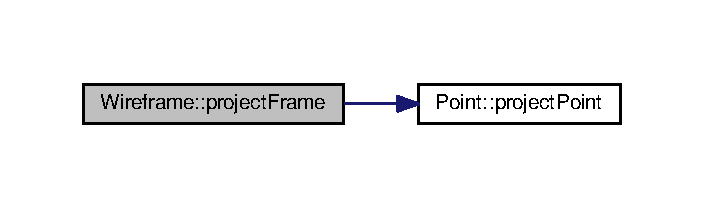
\includegraphics[width=338pt]{class_wireframe_a3ed1a5c8abc099d1eea1495b3b87e52e_cgraph}
\end{center}
\end{figure}


\index{Wireframe@{Wireframe}!rotate\+Frame@{rotate\+Frame}}
\index{rotate\+Frame@{rotate\+Frame}!Wireframe@{Wireframe}}
\subsubsection[{\texorpdfstring{rotate\+Frame(int)}{rotateFrame(int)}}]{\setlength{\rightskip}{0pt plus 5cm}int Wireframe\+::rotate\+Frame (
\begin{DoxyParamCaption}
\item[{int}]{type}
\end{DoxyParamCaption}
)}\hypertarget{class_wireframe_ad3fbb29a285e80d4d3448ea4e3e96d93}{}\label{class_wireframe_ad3fbb29a285e80d4d3448ea4e3e96d93}
Rotate the \hyperlink{class_wireframe}{Wireframe} by ten degrees

\subsection{Friends And Related Function Documentation}
\index{Wireframe@{Wireframe}!operator$<$$<$@{operator$<$$<$}}
\index{operator$<$$<$@{operator$<$$<$}!Wireframe@{Wireframe}}
\subsubsection[{\texorpdfstring{operator$<$$<$}{operator<<}}]{\setlength{\rightskip}{0pt plus 5cm}std\+::ostream\& operator$<$$<$ (
\begin{DoxyParamCaption}
\item[{std\+::ostream \&}]{out, }
\item[{const {\bf Wireframe} \&}]{op}
\end{DoxyParamCaption}
)\hspace{0.3cm}{\ttfamily [friend]}}\hypertarget{class_wireframe_ad074337c71dffaa7d1c65bf7ddf23e0e}{}\label{class_wireframe_ad074337c71dffaa7d1c65bf7ddf23e0e}


\subsection{Member Data Documentation}
\index{Wireframe@{Wireframe}!adjacency\+Matrix@{adjacency\+Matrix}}
\index{adjacency\+Matrix@{adjacency\+Matrix}!Wireframe@{Wireframe}}
\subsubsection[{\texorpdfstring{adjacency\+Matrix}{adjacencyMatrix}}]{\setlength{\rightskip}{0pt plus 5cm}vector$<$vector$<$int$>$ $>$ Wireframe\+::adjacency\+Matrix}\hypertarget{class_wireframe_a0bd14f3c6be92f087fddbbe7e4ddc344}{}\label{class_wireframe_a0bd14f3c6be92f087fddbbe7e4ddc344}
\index{Wireframe@{Wireframe}!edges@{edges}}
\index{edges@{edges}!Wireframe@{Wireframe}}
\subsubsection[{\texorpdfstring{edges}{edges}}]{\setlength{\rightskip}{0pt plus 5cm}vector$<${\bf Edge}$>$ Wireframe\+::edges}\hypertarget{class_wireframe_aef6867295610ed6d02a40c3e3b27700e}{}\label{class_wireframe_aef6867295610ed6d02a40c3e3b27700e}
\index{Wireframe@{Wireframe}!vertices@{vertices}}
\index{vertices@{vertices}!Wireframe@{Wireframe}}
\subsubsection[{\texorpdfstring{vertices}{vertices}}]{\setlength{\rightskip}{0pt plus 5cm}vector$<${\bf Point}$>$ Wireframe\+::vertices}\hypertarget{class_wireframe_a8a327766b43c4260925c0bacab853d02}{}\label{class_wireframe_a8a327766b43c4260925c0bacab853d02}


The documentation for this class was generated from the following files\+:\begin{DoxyCompactItemize}
\item 
Packag\+E\+D/include/\hyperlink{_classes_8h}{Classes.\+h}\item 
Packag\+E\+D/src/\hyperlink{_wireframe_8cpp}{Wireframe.\+cpp}\end{DoxyCompactItemize}

\chapter{File Documentation}
\section{G\+:/compu/\+C\+O\+P290/\+Packag\+E\+D/include/\+Classes.h File Reference}
\label{include_2_classes_8h}\index{G\+:/compu/\+C\+O\+P290/\+Packag\+E\+D/include/\+Classes.\+h@{G\+:/compu/\+C\+O\+P290/\+Packag\+E\+D/include/\+Classes.\+h}}
\subsection*{Classes}
\begin{DoxyCompactItemize}
\item 
class \textbf{ Point}
\item 
class \textbf{ Edge}
\item 
class \textbf{ Face}
\item 
class \textbf{ Ortho\+Projection}
\item 
class \textbf{ Wireframe}
\end{DoxyCompactItemize}

\section{G\+:/compu/\+C\+O\+P290/\+Packag\+E\+D/src/\+Classes.h File Reference}
\label{src_2_classes_8h}\index{G\+:/compu/\+C\+O\+P290/\+Packag\+E\+D/src/\+Classes.\+h@{G\+:/compu/\+C\+O\+P290/\+Packag\+E\+D/src/\+Classes.\+h}}
\subsection*{Classes}
\begin{DoxyCompactItemize}
\item 
class \textbf{ Point}
\item 
class \textbf{ Edge}
\item 
class \textbf{ Face}
\item 
class \textbf{ Ortho\+Projection}
\item 
class \textbf{ Wireframe}
\end{DoxyCompactItemize}

\section{G\+:/compu/\+C\+O\+P290/\+Packag\+E\+D/\+R\+E\+A\+D\+ME.md File Reference}
\label{_r_e_a_d_m_e_8md}\index{G\+:/compu/\+C\+O\+P290/\+Packag\+E\+D/\+R\+E\+A\+D\+M\+E.\+md@{G\+:/compu/\+C\+O\+P290/\+Packag\+E\+D/\+R\+E\+A\+D\+M\+E.\+md}}

\section{G\+:/compu/\+C\+O\+P290/\+Packag\+E\+D/src/check.cpp File Reference}
\label{check_8cpp}\index{G\+:/compu/\+C\+O\+P290/\+Packag\+E\+D/src/check.\+cpp@{G\+:/compu/\+C\+O\+P290/\+Packag\+E\+D/src/check.\+cpp}}
{\ttfamily \#include $<$iostream$>$}\newline
\subsection*{Classes}
\begin{DoxyCompactItemize}
\item 
class \textbf{ check}
\end{DoxyCompactItemize}
\subsection*{Functions}
\begin{DoxyCompactItemize}
\item 
int \textbf{ function} (int[4])
\item 
int $\ast$ \textbf{ check\+Array\+Pointer} ()
\item 
int \textbf{ main} ()
\item 
int \textbf{ function} (int arr[$\,$])
\end{DoxyCompactItemize}
\subsection*{Variables}
\begin{DoxyCompactItemize}
\item 
class \textbf{ check} \textbf{ check1}
\end{DoxyCompactItemize}


\subsection{Function Documentation}
\mbox{\label{check_8cpp_a8874c37ad048edac27dd2fbdcd710024}} 
\index{check.\+cpp@{check.\+cpp}!check\+Array\+Pointer@{check\+Array\+Pointer}}
\index{check\+Array\+Pointer@{check\+Array\+Pointer}!check.\+cpp@{check.\+cpp}}
\subsubsection{check\+Array\+Pointer()}
{\footnotesize\ttfamily int $\ast$ check\+Array\+Pointer (\begin{DoxyParamCaption}{ }\end{DoxyParamCaption})}

\mbox{\label{check_8cpp_a527432c71d7bedc5261d8b3834fc5266}} 
\index{check.\+cpp@{check.\+cpp}!function@{function}}
\index{function@{function}!check.\+cpp@{check.\+cpp}}
\subsubsection{function()\hspace{0.1cm}{\footnotesize\ttfamily [1/2]}}
{\footnotesize\ttfamily int function (\begin{DoxyParamCaption}\item[{int}]{[4] }\end{DoxyParamCaption})}

\mbox{\label{check_8cpp_aa3c75eb137ff09226af29ac28246c2fa}} 
\index{check.\+cpp@{check.\+cpp}!function@{function}}
\index{function@{function}!check.\+cpp@{check.\+cpp}}
\subsubsection{function()\hspace{0.1cm}{\footnotesize\ttfamily [2/2]}}
{\footnotesize\ttfamily int function (\begin{DoxyParamCaption}\item[{int}]{arr[$\,$] }\end{DoxyParamCaption})}

\mbox{\label{check_8cpp_ae66f6b31b5ad750f1fe042a706a4e3d4}} 
\index{check.\+cpp@{check.\+cpp}!main@{main}}
\index{main@{main}!check.\+cpp@{check.\+cpp}}
\subsubsection{main()}
{\footnotesize\ttfamily int main (\begin{DoxyParamCaption}{ }\end{DoxyParamCaption})}



\subsection{Variable Documentation}
\mbox{\label{check_8cpp_a0eac68a12bc6181ee5265149c4db0a02}} 
\index{check.\+cpp@{check.\+cpp}!check1@{check1}}
\index{check1@{check1}!check.\+cpp@{check.\+cpp}}
\subsubsection{check1}
{\footnotesize\ttfamily class \textbf{ check}  check1}


\hypertarget{_main_8cpp}{}\section{Packag\+E\+D/src/\+Main.cpp File Reference}
\label{_main_8cpp}\index{Packag\+E\+D/src/\+Main.\+cpp@{Packag\+E\+D/src/\+Main.\+cpp}}
{\ttfamily \#include $<$iostream$>$}\\*
{\ttfamily \#include $<$vector$>$}\\*
{\ttfamily \#include $<$Eigen/\+Dense$>$}\\*
{\ttfamily \#include $<$gtkmm.\+h$>$}\\*
{\ttfamily \#include \char`\"{}gui.\+h\char`\"{}}\\*
{\ttfamily \#include $<$fstream$>$}\\*
Include dependency graph for Main.\+cpp\+:\nopagebreak
\begin{figure}[H]
\begin{center}
\leavevmode
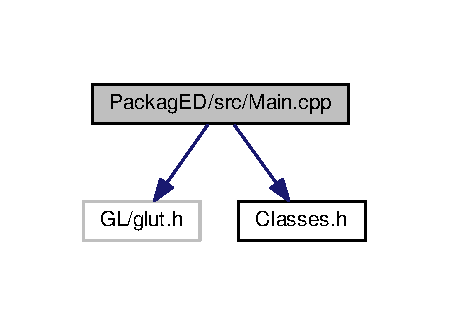
\includegraphics[width=350pt]{_main_8cpp__incl}
\end{center}
\end{figure}
\subsection*{Functions}
\begin{DoxyCompactItemize}
\item 
int \hyperlink{_main_8cpp_a0ddf1224851353fc92bfbff6f499fa97}{main} (int argc, char $\ast$argv\mbox{[}$\,$\mbox{]})
\item 
int \hyperlink{_main_8cpp_a1c78b5af1e79bd9d8c8660a677d8379d}{check3D} ()
\item 
\hyperlink{class_plane_projection}{Plane\+Projection} $\ast$ \hyperlink{_main_8cpp_ac40e3d324848f2c969794764a35076c1}{input3\+Dfile} (string filename)
\item 
int \hyperlink{_main_8cpp_af55dca22c340b42a2992f9f270495789}{check2D} ()
\item 
\hyperlink{class_wireframe}{Wireframe} $\ast$ \hyperlink{_main_8cpp_a58dea5abaabfe7848670218ba390150a}{input2\+Dfile} (string filename)
\item 
\hyperlink{class_plane_projection}{Plane\+Projection} $\ast$ \hyperlink{_main_8cpp_acab27e3306ac9a4a308e62f633e30e84}{create\+Object} (\hyperlink{class_object3_d}{Object3D} $\ast$object, double plane\mbox{[}4\mbox{]})
\item 
\hyperlink{class_wireframe}{Wireframe} $\ast$ \hyperlink{_main_8cpp_aa5092f55af8fcb978372a0bf77aa69f6}{create\+Projection} (\hyperlink{class_projection2_d}{Projection2D} $\ast$projection)
\end{DoxyCompactItemize}


\subsection{Function Documentation}
\index{Main.\+cpp@{Main.\+cpp}!check2D@{check2D}}
\index{check2D@{check2D}!Main.\+cpp@{Main.\+cpp}}
\subsubsection[{\texorpdfstring{check2\+D()}{check2D()}}]{\setlength{\rightskip}{0pt plus 5cm}int check2D (
\begin{DoxyParamCaption}
{}
\end{DoxyParamCaption}
)}\hypertarget{_main_8cpp_af55dca22c340b42a2992f9f270495789}{}\label{_main_8cpp_af55dca22c340b42a2992f9f270495789}


Here is the call graph for this function\+:\nopagebreak
\begin{figure}[H]
\begin{center}
\leavevmode
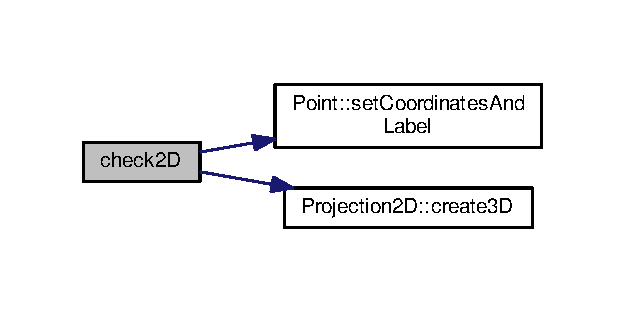
\includegraphics[width=300pt]{_main_8cpp_af55dca22c340b42a2992f9f270495789_cgraph}
\end{center}
\end{figure}


\index{Main.\+cpp@{Main.\+cpp}!check3D@{check3D}}
\index{check3D@{check3D}!Main.\+cpp@{Main.\+cpp}}
\subsubsection[{\texorpdfstring{check3\+D()}{check3D()}}]{\setlength{\rightskip}{0pt plus 5cm}int check3D (
\begin{DoxyParamCaption}
{}
\end{DoxyParamCaption}
)}\hypertarget{_main_8cpp_a1c78b5af1e79bd9d8c8660a677d8379d}{}\label{_main_8cpp_a1c78b5af1e79bd9d8c8660a677d8379d}


Here is the call graph for this function\+:\nopagebreak
\begin{figure}[H]
\begin{center}
\leavevmode
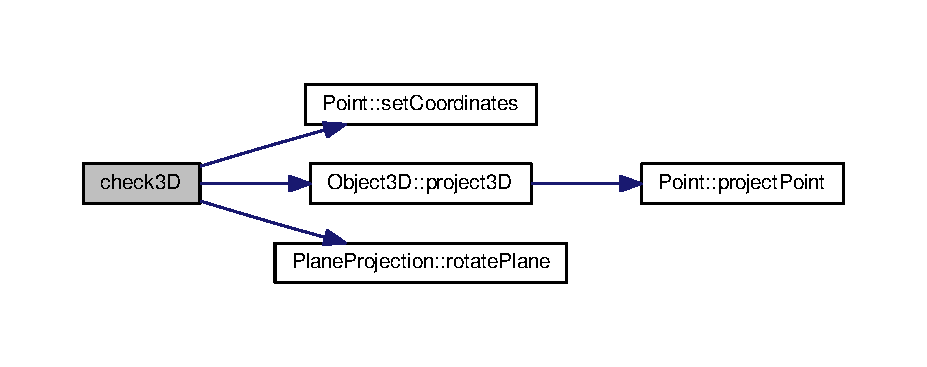
\includegraphics[width=350pt]{_main_8cpp_a1c78b5af1e79bd9d8c8660a677d8379d_cgraph}
\end{center}
\end{figure}


\index{Main.\+cpp@{Main.\+cpp}!create\+Object@{create\+Object}}
\index{create\+Object@{create\+Object}!Main.\+cpp@{Main.\+cpp}}
\subsubsection[{\texorpdfstring{create\+Object(\+Object3\+D $\ast$object, double plane[4])}{createObject(Object3D *object, double plane[4])}}]{\setlength{\rightskip}{0pt plus 5cm}{\bf Plane\+Projection}$\ast$ create\+Object (
\begin{DoxyParamCaption}
\item[{{\bf Object3D} $\ast$}]{object, }
\item[{double}]{plane\mbox{[}4\mbox{]}}
\end{DoxyParamCaption}
)}\hypertarget{_main_8cpp_acab27e3306ac9a4a308e62f633e30e84}{}\label{_main_8cpp_acab27e3306ac9a4a308e62f633e30e84}
This function shall make use of the gtk library, to interactively take input from the user and returns the 3D object created from the user input

Here is the call graph for this function\+:\nopagebreak
\begin{figure}[H]
\begin{center}
\leavevmode
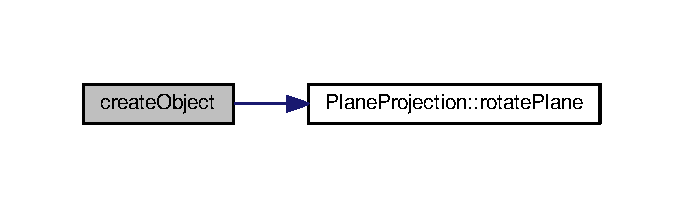
\includegraphics[width=328pt]{_main_8cpp_acab27e3306ac9a4a308e62f633e30e84_cgraph}
\end{center}
\end{figure}


\index{Main.\+cpp@{Main.\+cpp}!create\+Projection@{create\+Projection}}
\index{create\+Projection@{create\+Projection}!Main.\+cpp@{Main.\+cpp}}
\subsubsection[{\texorpdfstring{create\+Projection(\+Projection2\+D $\ast$projection)}{createProjection(Projection2D *projection)}}]{\setlength{\rightskip}{0pt plus 5cm}{\bf Wireframe}$\ast$ create\+Projection (
\begin{DoxyParamCaption}
\item[{{\bf Projection2D} $\ast$}]{projection}
\end{DoxyParamCaption}
)}\hypertarget{_main_8cpp_aa5092f55af8fcb978372a0bf77aa69f6}{}\label{_main_8cpp_aa5092f55af8fcb978372a0bf77aa69f6}
This function shall make use of the gtk library, to interactively take input from the user, to form a 2D projection and returns the Projection created from the user input

Here is the call graph for this function\+:\nopagebreak
\begin{figure}[H]
\begin{center}
\leavevmode
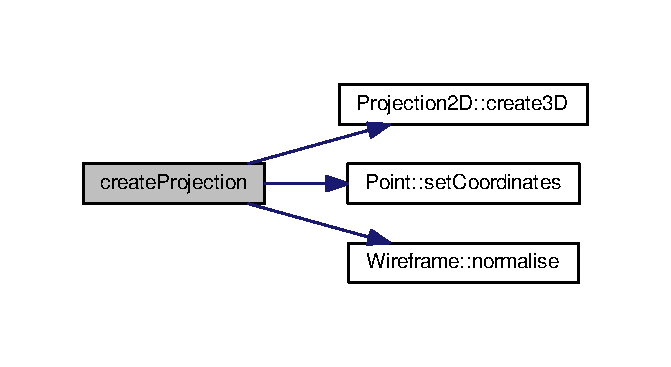
\includegraphics[width=322pt]{_main_8cpp_aa5092f55af8fcb978372a0bf77aa69f6_cgraph}
\end{center}
\end{figure}


\index{Main.\+cpp@{Main.\+cpp}!input2\+Dfile@{input2\+Dfile}}
\index{input2\+Dfile@{input2\+Dfile}!Main.\+cpp@{Main.\+cpp}}
\subsubsection[{\texorpdfstring{input2\+Dfile(string filename)}{input2Dfile(string filename)}}]{\setlength{\rightskip}{0pt plus 5cm}{\bf Wireframe}$\ast$ input2\+Dfile (
\begin{DoxyParamCaption}
\item[{string}]{filename}
\end{DoxyParamCaption}
)}\hypertarget{_main_8cpp_a58dea5abaabfe7848670218ba390150a}{}\label{_main_8cpp_a58dea5abaabfe7848670218ba390150a}
Function to get input of 2D Projections from a file

Here is the call graph for this function\+:\nopagebreak
\begin{figure}[H]
\begin{center}
\leavevmode
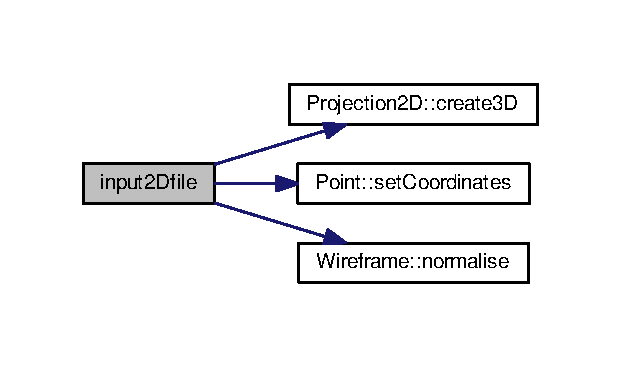
\includegraphics[width=298pt]{_main_8cpp_a58dea5abaabfe7848670218ba390150a_cgraph}
\end{center}
\end{figure}


\index{Main.\+cpp@{Main.\+cpp}!input3\+Dfile@{input3\+Dfile}}
\index{input3\+Dfile@{input3\+Dfile}!Main.\+cpp@{Main.\+cpp}}
\subsubsection[{\texorpdfstring{input3\+Dfile(string filename)}{input3Dfile(string filename)}}]{\setlength{\rightskip}{0pt plus 5cm}{\bf Plane\+Projection}$\ast$ input3\+Dfile (
\begin{DoxyParamCaption}
\item[{string}]{filename}
\end{DoxyParamCaption}
)}\hypertarget{_main_8cpp_ac40e3d324848f2c969794764a35076c1}{}\label{_main_8cpp_ac40e3d324848f2c969794764a35076c1}
Function to get input of the 3D Object from file

Here is the call graph for this function\+:\nopagebreak
\begin{figure}[H]
\begin{center}
\leavevmode
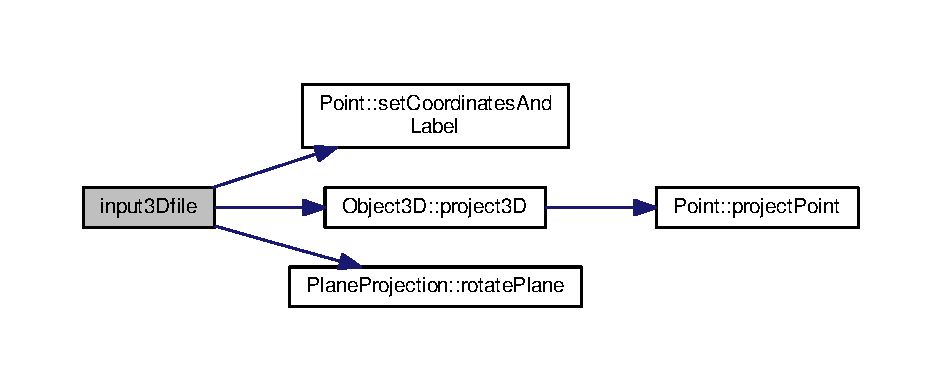
\includegraphics[width=350pt]{_main_8cpp_ac40e3d324848f2c969794764a35076c1_cgraph}
\end{center}
\end{figure}


\index{Main.\+cpp@{Main.\+cpp}!main@{main}}
\index{main@{main}!Main.\+cpp@{Main.\+cpp}}
\subsubsection[{\texorpdfstring{main(int argc, char $\ast$argv[])}{main(int argc, char *argv[])}}]{\setlength{\rightskip}{0pt plus 5cm}int main (
\begin{DoxyParamCaption}
\item[{int}]{argc, }
\item[{char $\ast$}]{argv\mbox{[}$\,$\mbox{]}}
\end{DoxyParamCaption}
)}\hypertarget{_main_8cpp_a0ddf1224851353fc92bfbff6f499fa97}{}\label{_main_8cpp_a0ddf1224851353fc92bfbff6f499fa97}
The main function shall be responsible for calling various other functions and instantiating the classes for using their functions cop290
\hypertarget{_object3_d_8cpp}{}\section{Packag\+E\+D/src/\+Object3D.cpp File Reference}
\label{_object3_d_8cpp}\index{Packag\+E\+D/src/\+Object3\+D.\+cpp@{Packag\+E\+D/src/\+Object3\+D.\+cpp}}
{\ttfamily \#include \char`\"{}Classes.\+h\char`\"{}}\\*

\hypertarget{_ortho_projection_8cpp}{}\section{Packag\+E\+D/src/\+Ortho\+Projection.cpp File Reference}
\label{_ortho_projection_8cpp}\index{Packag\+E\+D/src/\+Ortho\+Projection.\+cpp@{Packag\+E\+D/src/\+Ortho\+Projection.\+cpp}}
{\ttfamily \#include \char`\"{}Classes.\+h\char`\"{}}\\*

\hypertarget{_point_8cpp}{}\section{Packag\+E\+D/src/\+Point.cpp File Reference}
\label{_point_8cpp}\index{Packag\+E\+D/src/\+Point.\+cpp@{Packag\+E\+D/src/\+Point.\+cpp}}
{\ttfamily \#include $<$iostream$>$}\\*
{\ttfamily \#include \char`\"{}Classes.\+h\char`\"{}}\\*
Include dependency graph for Point.\+cpp\+:
\nopagebreak
\begin{figure}[H]
\begin{center}
\leavevmode
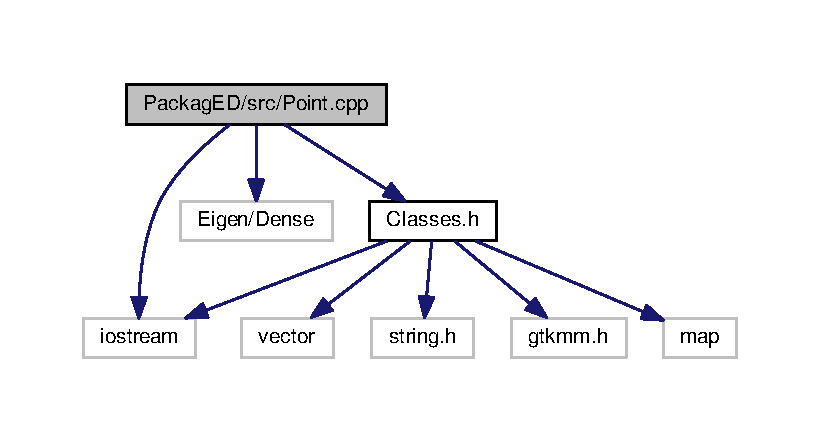
\includegraphics[width=214pt]{_point_8cpp__incl}
\end{center}
\end{figure}

\hypertarget{_projection2_d_8cpp}{}\section{Packag\+E\+D/src/\+Projection2D.cpp File Reference}
\label{_projection2_d_8cpp}\index{Packag\+E\+D/src/\+Projection2\+D.\+cpp@{Packag\+E\+D/src/\+Projection2\+D.\+cpp}}
{\ttfamily \#include \char`\"{}Classes.\+h\char`\"{}}\\*
Include dependency graph for Projection2\+D.\+cpp\+:
\nopagebreak
\begin{figure}[H]
\begin{center}
\leavevmode
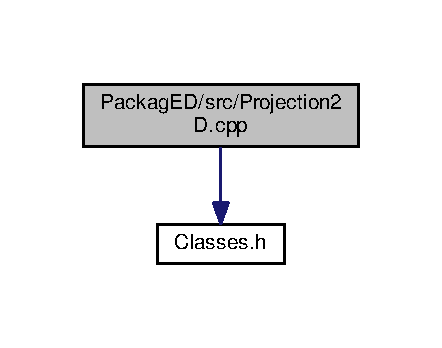
\includegraphics[width=212pt]{_projection2_d_8cpp__incl}
\end{center}
\end{figure}
\subsection*{Classes}
\begin{DoxyCompactItemize}
\item 
class \hyperlink{class_projection2_d}{Projection2D}
\end{DoxyCompactItemize}

%--- End generated contents ---

% Index
\backmatter
\newpage
\phantomsection
\clearemptydoublepage
\addcontentsline{toc}{chapter}{Index}
\printindex

\end{document}
